\documentclass{ximera}

\input{../../preamble.tex}

\author{}
\license{Creative Commons Attribution-ShareAlike 4.0 International License}
\acknowledgement{https://activecalculus.org/prelude/sec-changing-functions-models.html}

\begin{document}
\licenseAPC

Based on the graphs of $f(x)$ and $g(x)$ below, answer the following questions. 
\begin{center}
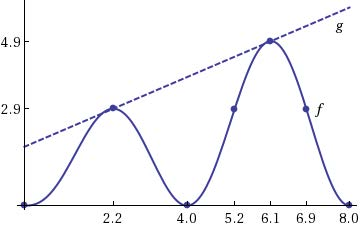
\includegraphics[width=1in]{WiaFgraphs10-1}
\end{center}
\begin{exercise}
Find $f(5.2)=\answer{2.9}$
\end{exercise}

\begin{exercise}
Fill in the blanks in each of the two points below to correctly complete the coordinates of two points on the graph of $g(x)$.
$$(6.1, \answer{4.9})$$
$$(\answer{2.2}, 2.9 )$$
\end{exercise}

\begin{exercise}
For how many value(s) of $x$ does $f(x)=2.9$?
$$\answer{3}$$
\end{exercise}

\begin{exercise}
For what value(s) of $x$ is/are $f(x)=2.9$? Enter in increasing order, one answer per box.
$$x=\answer{2.2}$$
$$x=\answer{5.2}$$
$$x=\answer{6.9}$$
\end{exercise}

\begin{exercise}
For how many value(s) of $x$ is/are $f(x)=g(x)$?
$$\answer{2}$$
\end{exercise}

\begin{exercise}
For what value(s) of $x$ is/are $f(x)=g(x)$? Enter in increasing order, one answer per box.
$$x=\answer{2.2}$$
$$x=\answer{6.1}$$
\end{exercise}

\end{document}
